\appendix
\chapter*{System Setup}
\label{chap:results}


%%%%%%%%%%%%%%%%%
%ASTRA
\begin{figure}[htp]
\begin{center}
{
  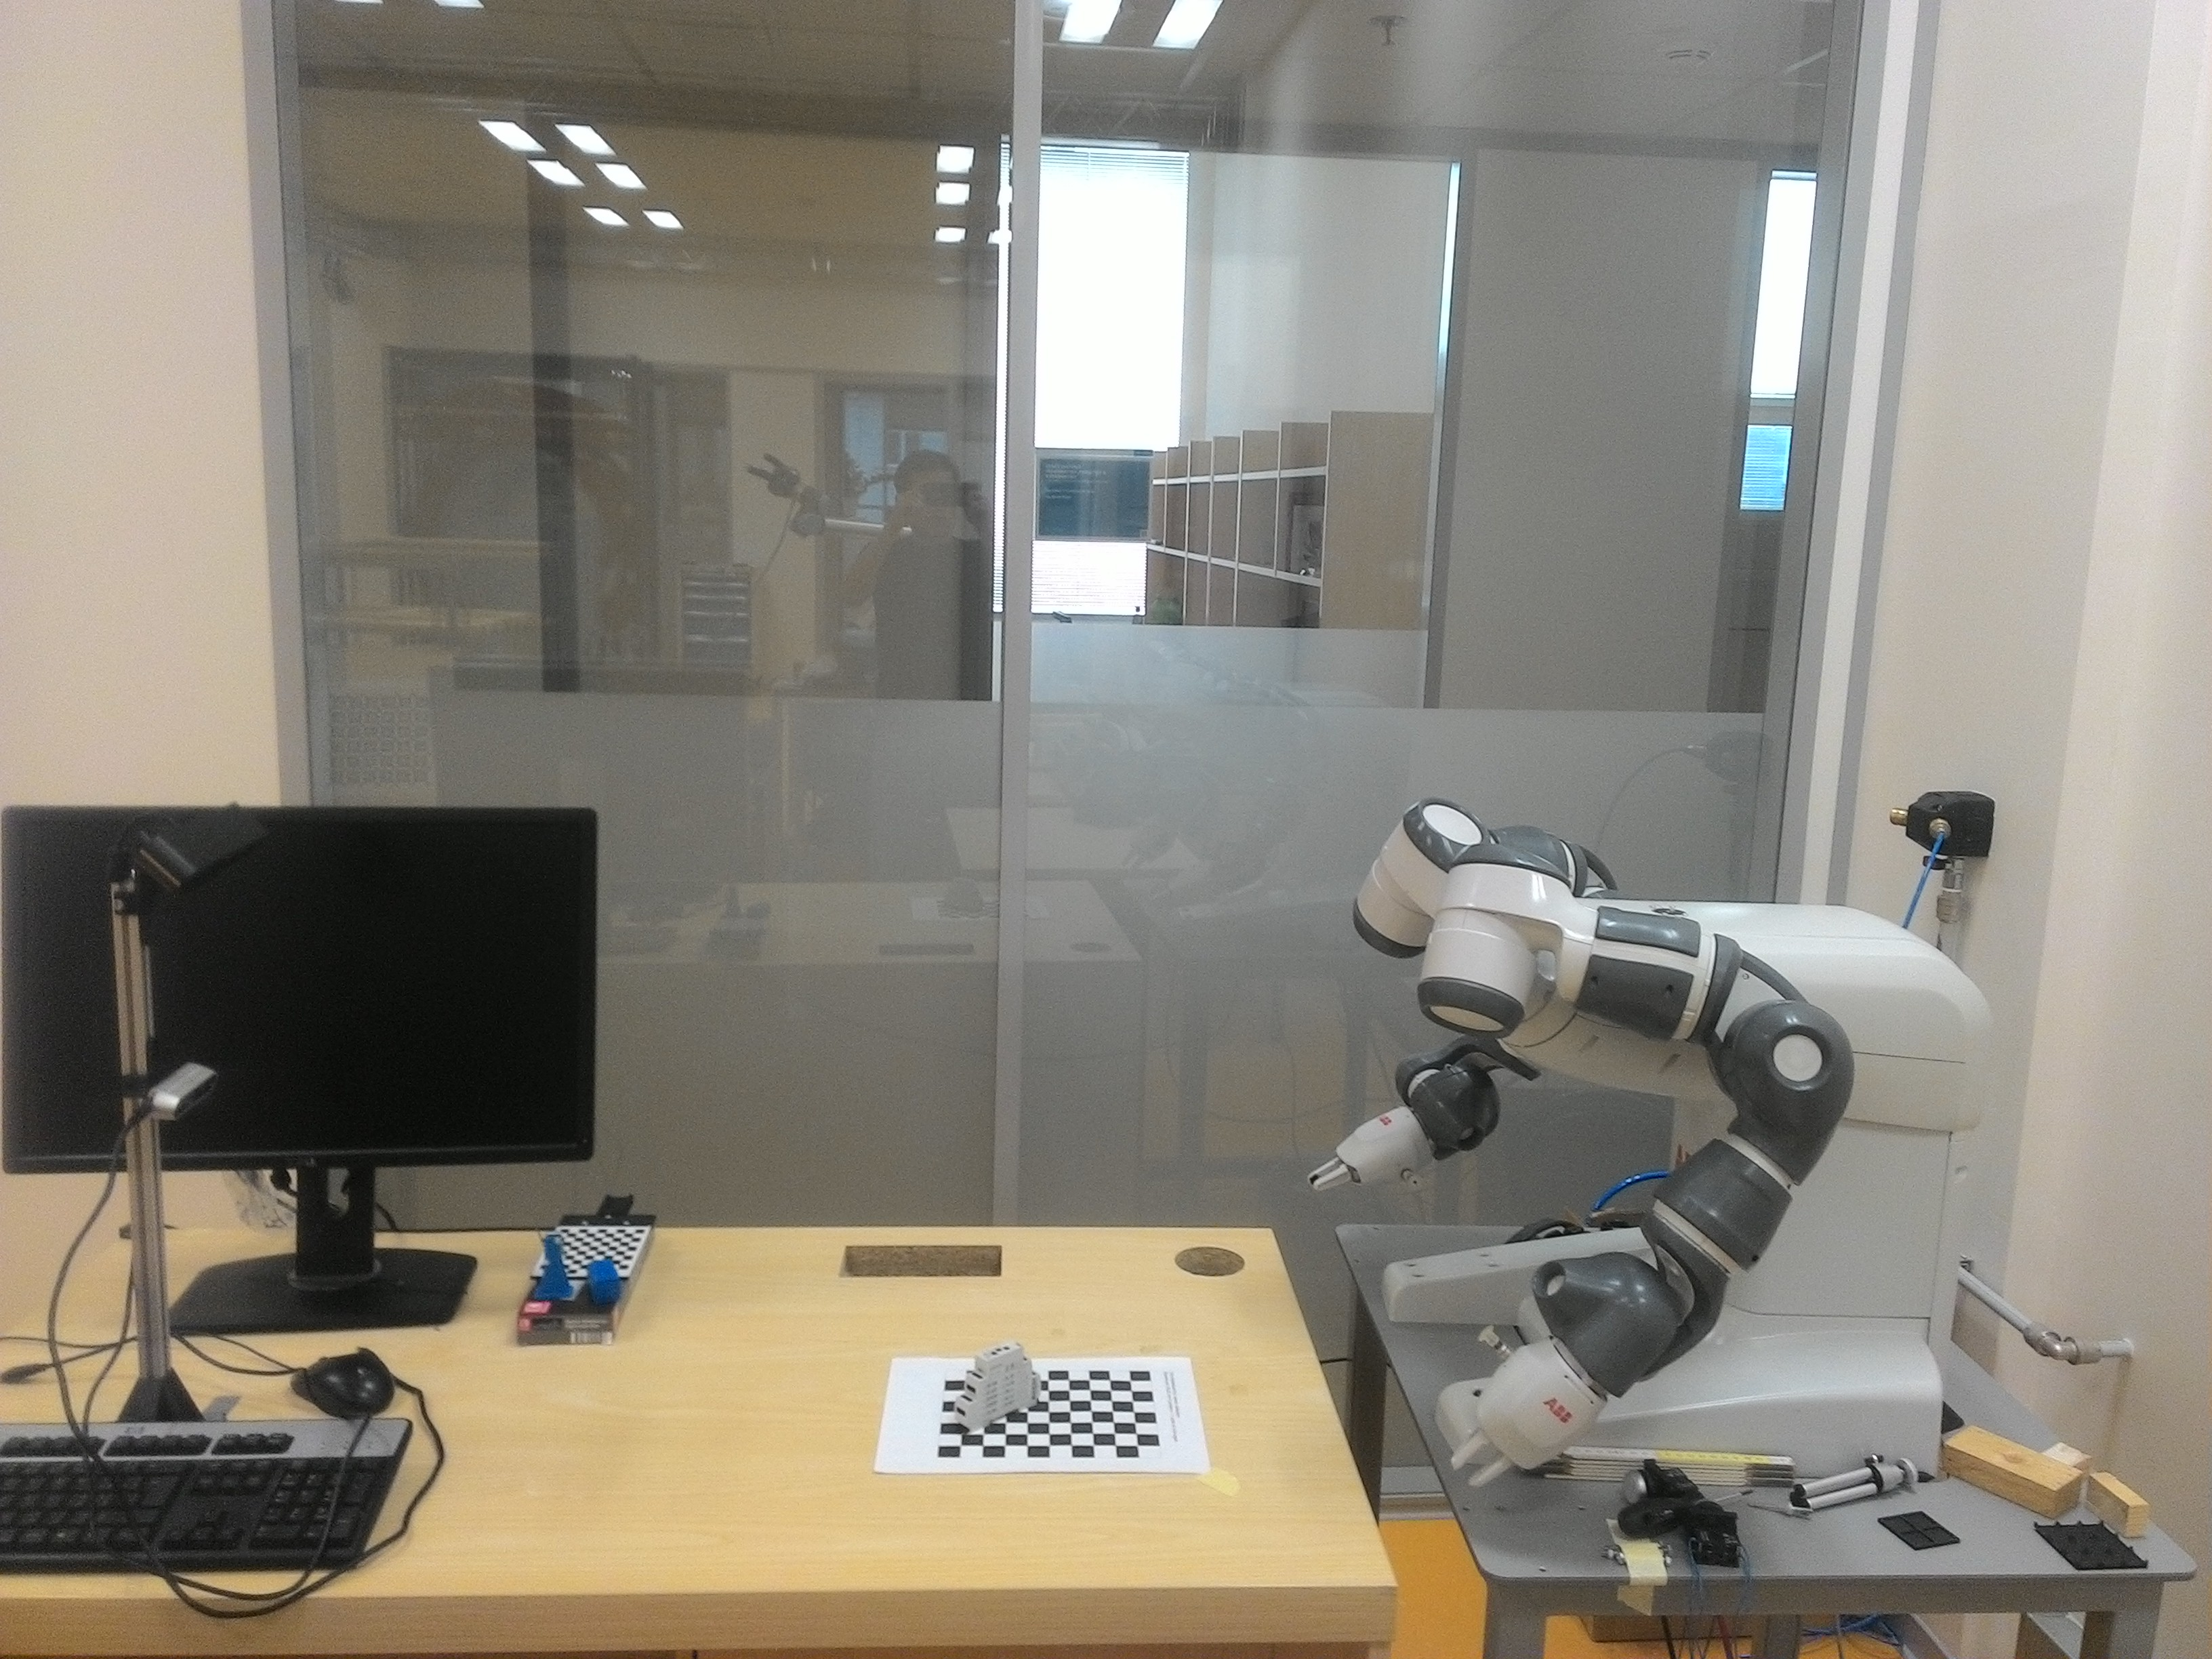
\includegraphics[clip,width=0.6\columnwidth]{images/setup1.jpg}
}
\end{center}
\begin{center}
{
  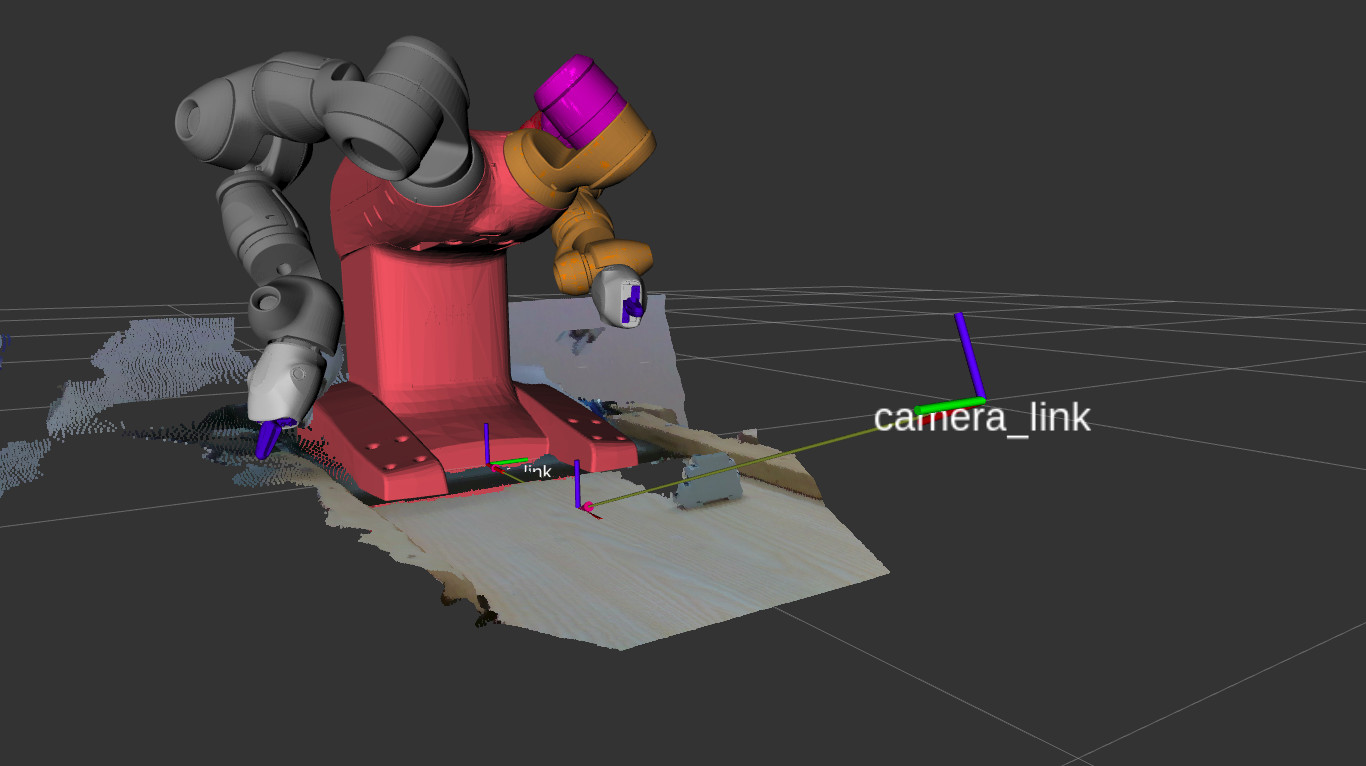
\includegraphics[clip,width=0.6\columnwidth]{images/system1.jpg}
}
\end{center}
\caption{Overview of the Validation System 1}
\label{setupsystem1}
\end{figure}




\begin{figure}[htp]
\begin{center}
{
  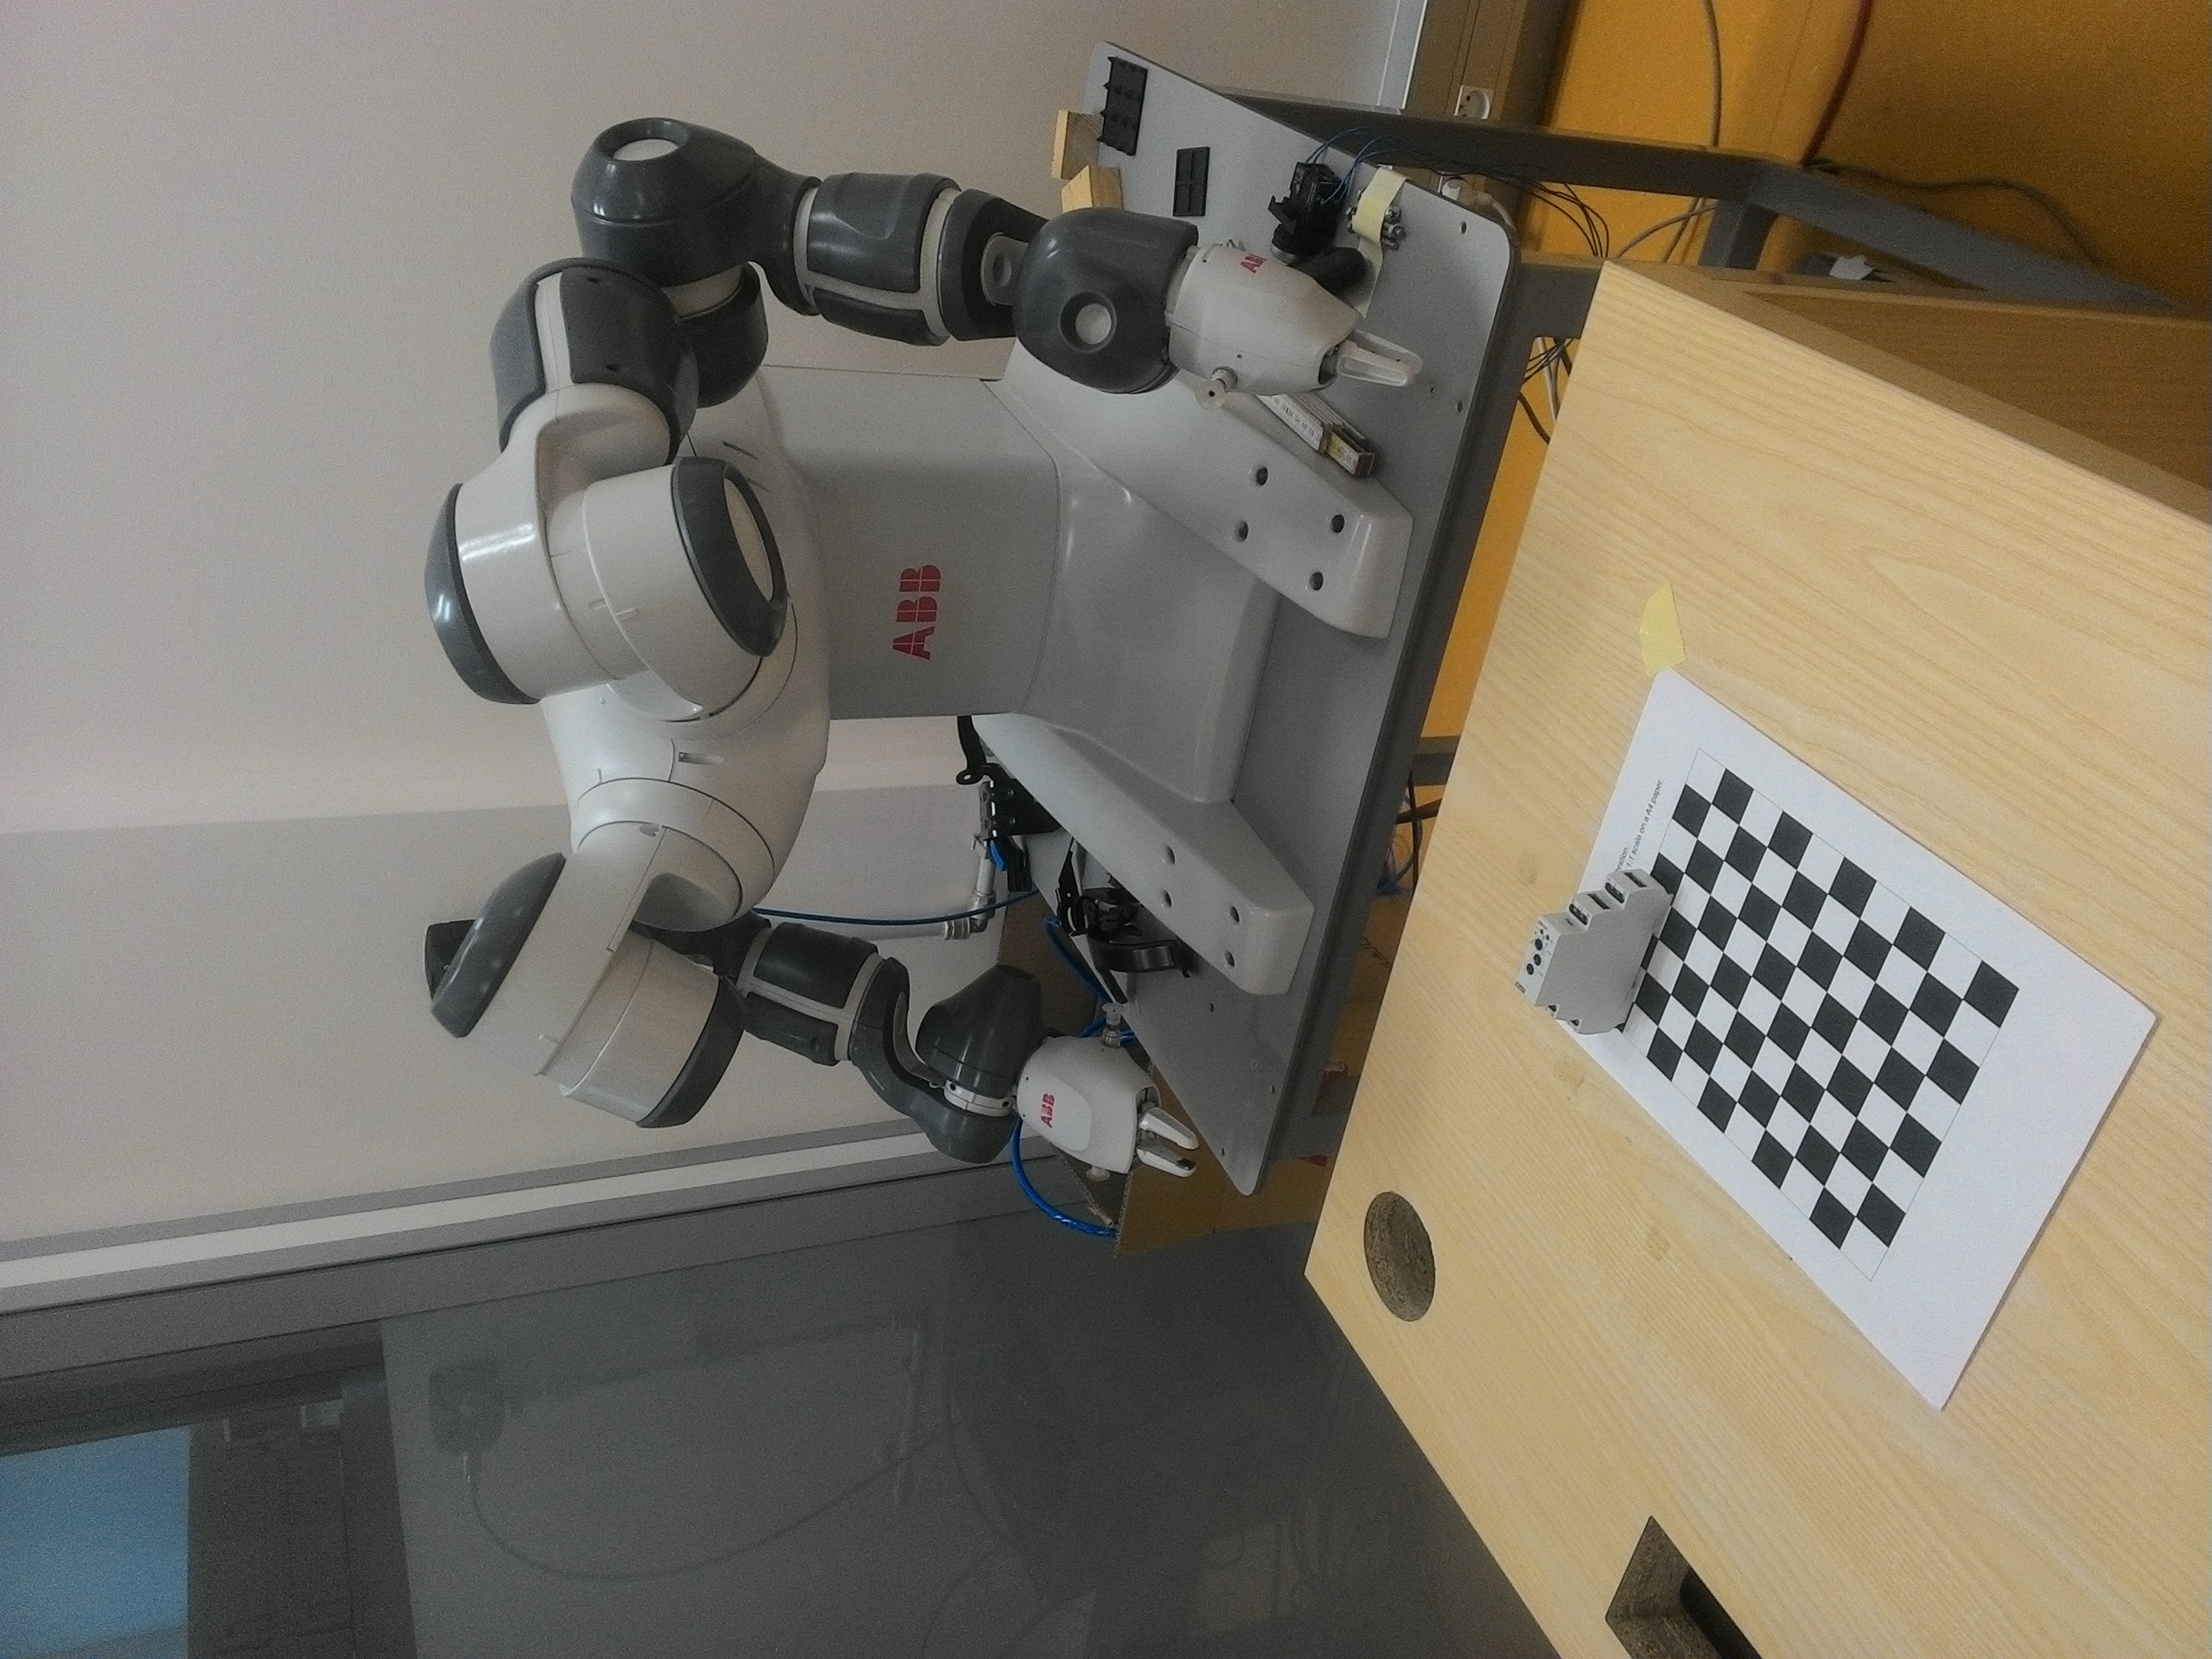
\includegraphics[clip,width=0.6\columnwidth]{images/setup2.png}
}
\end{center}
\begin{center}
{
  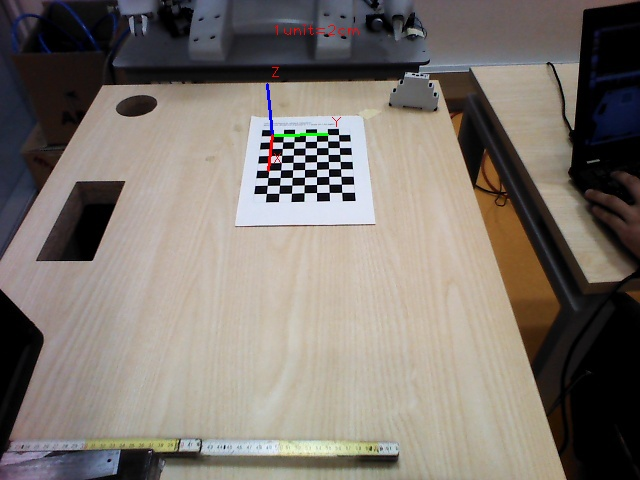
\includegraphics[clip,width=0.6\columnwidth]{images/setup3.jpg}
}
\end{center}
\caption{Overview of the Validation System 2}
\label{setupsystem2}
\end{figure}



%ASTRA
\begin{figure}[htp]
\begin{center}
{
  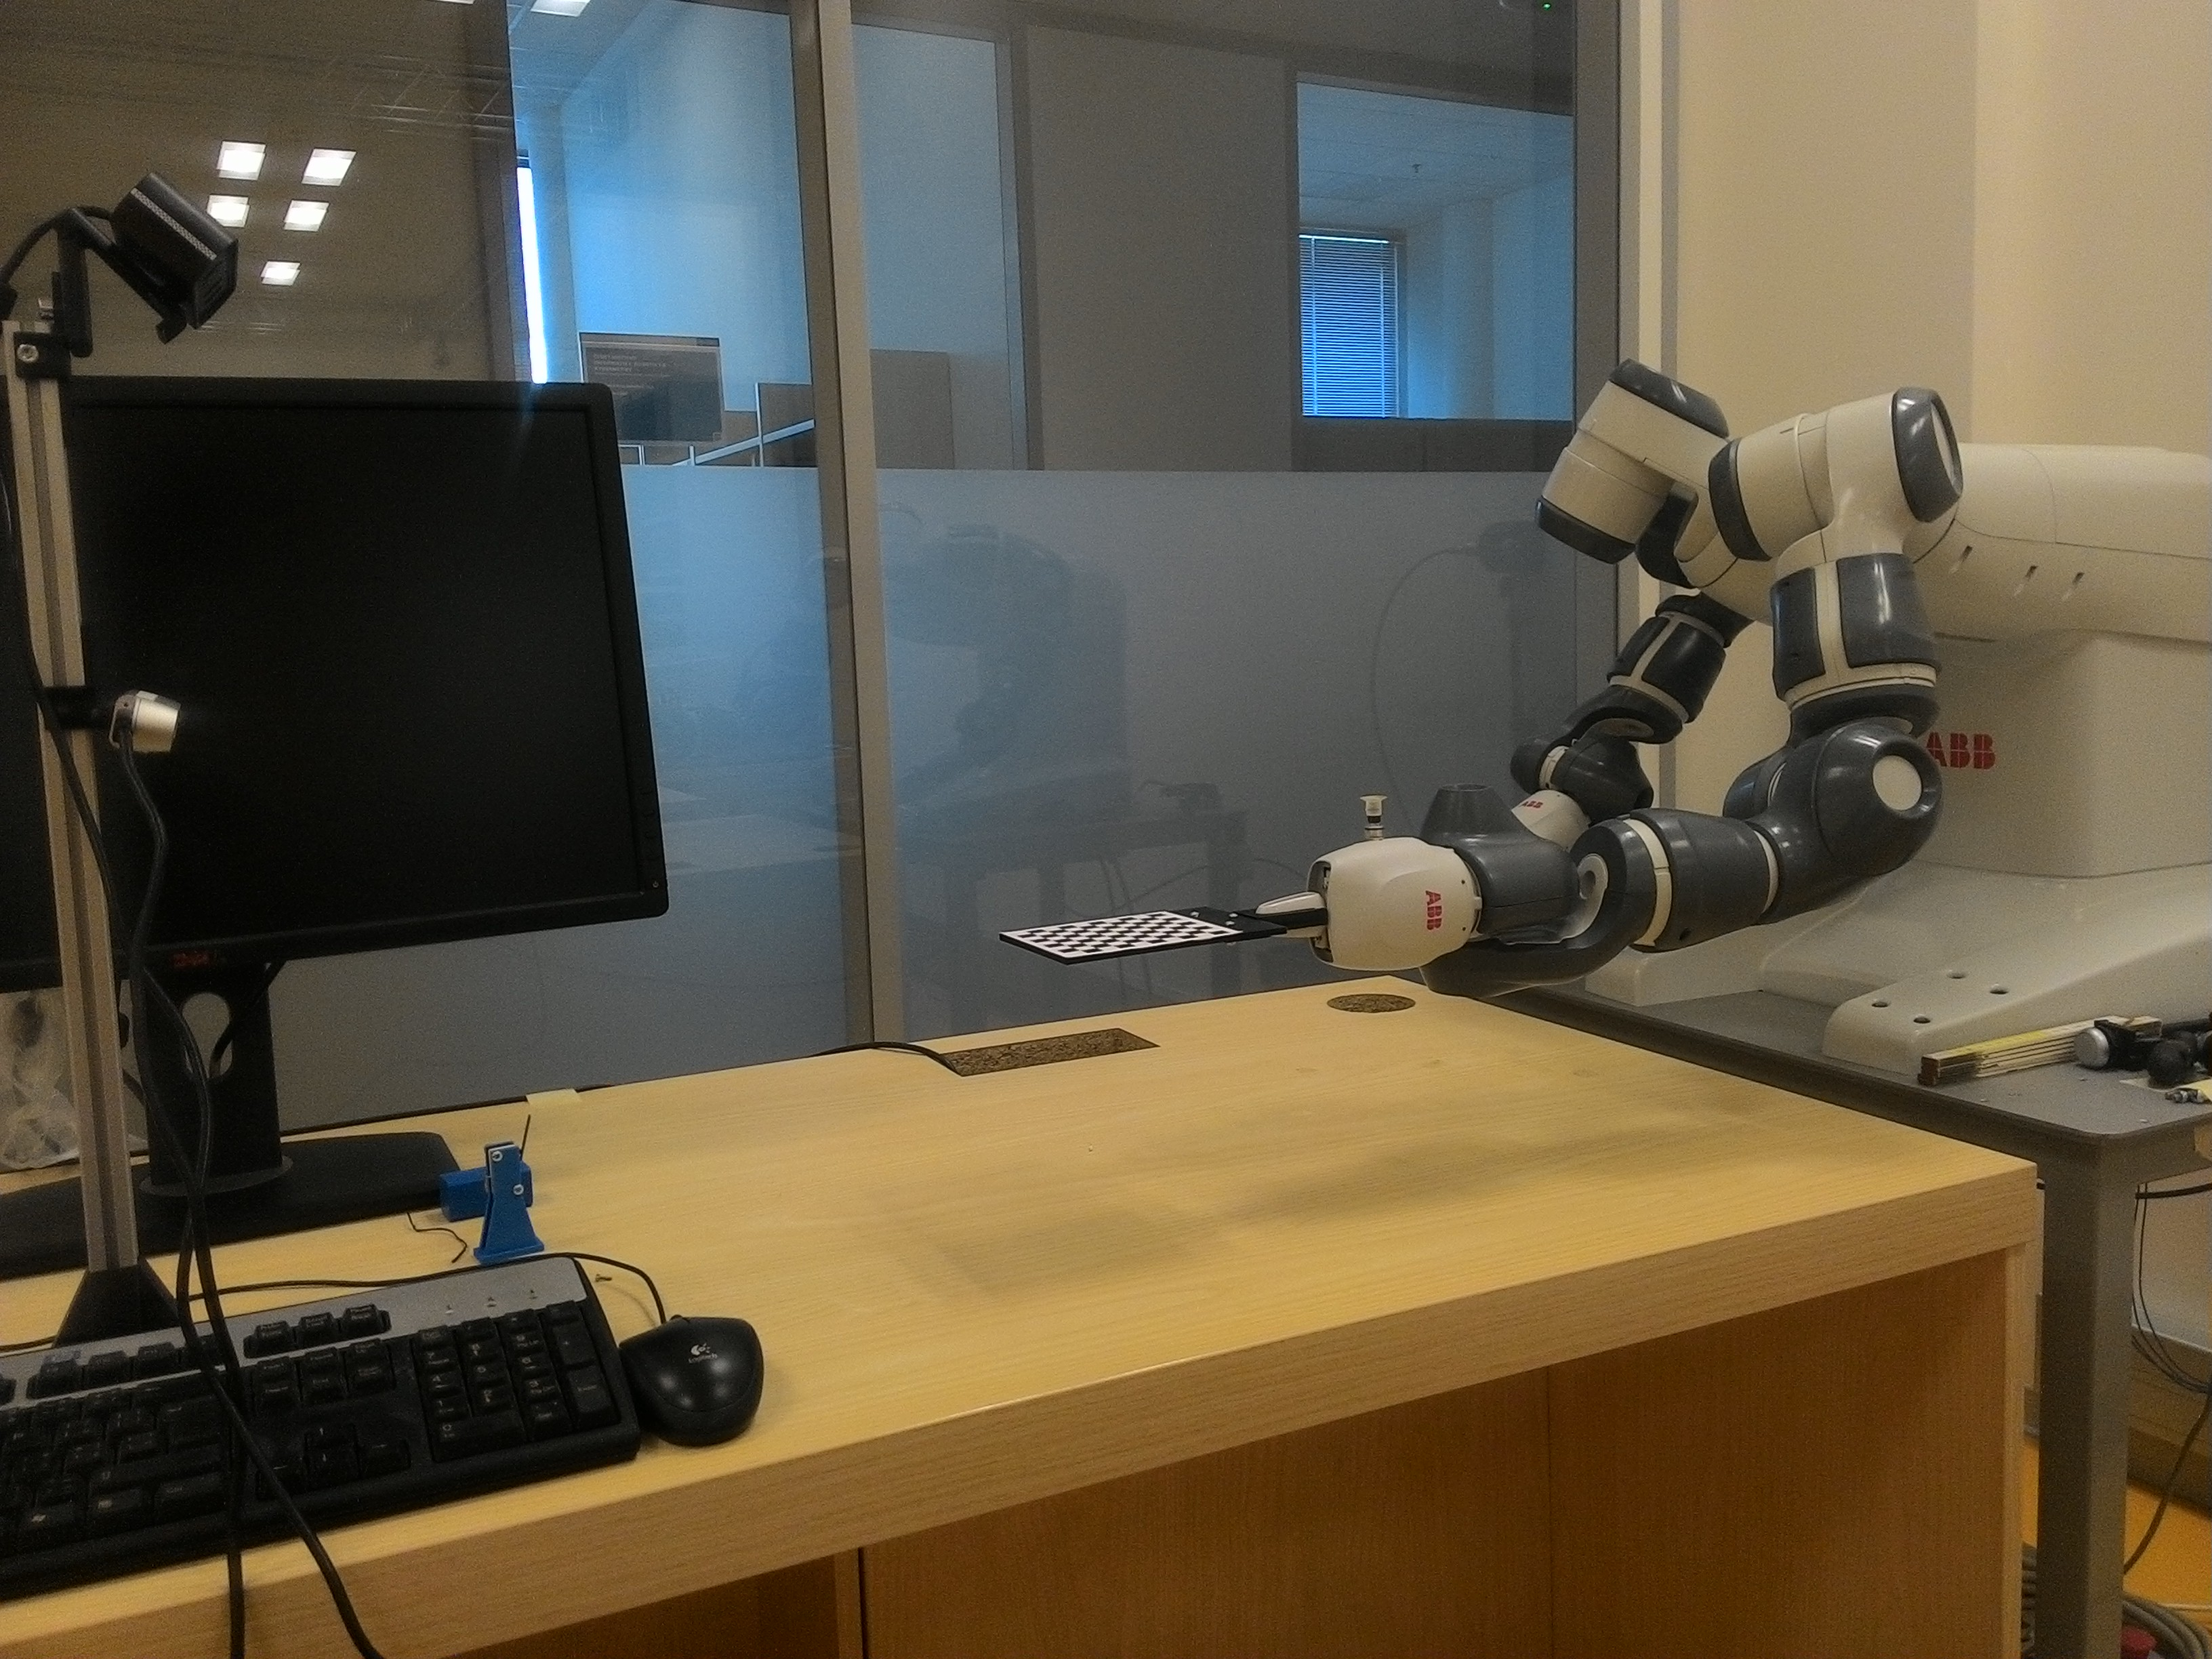
\includegraphics[clip,width=0.6\columnwidth]{images/ext1.jpg}
}
\end{center}
\begin{center}
{
  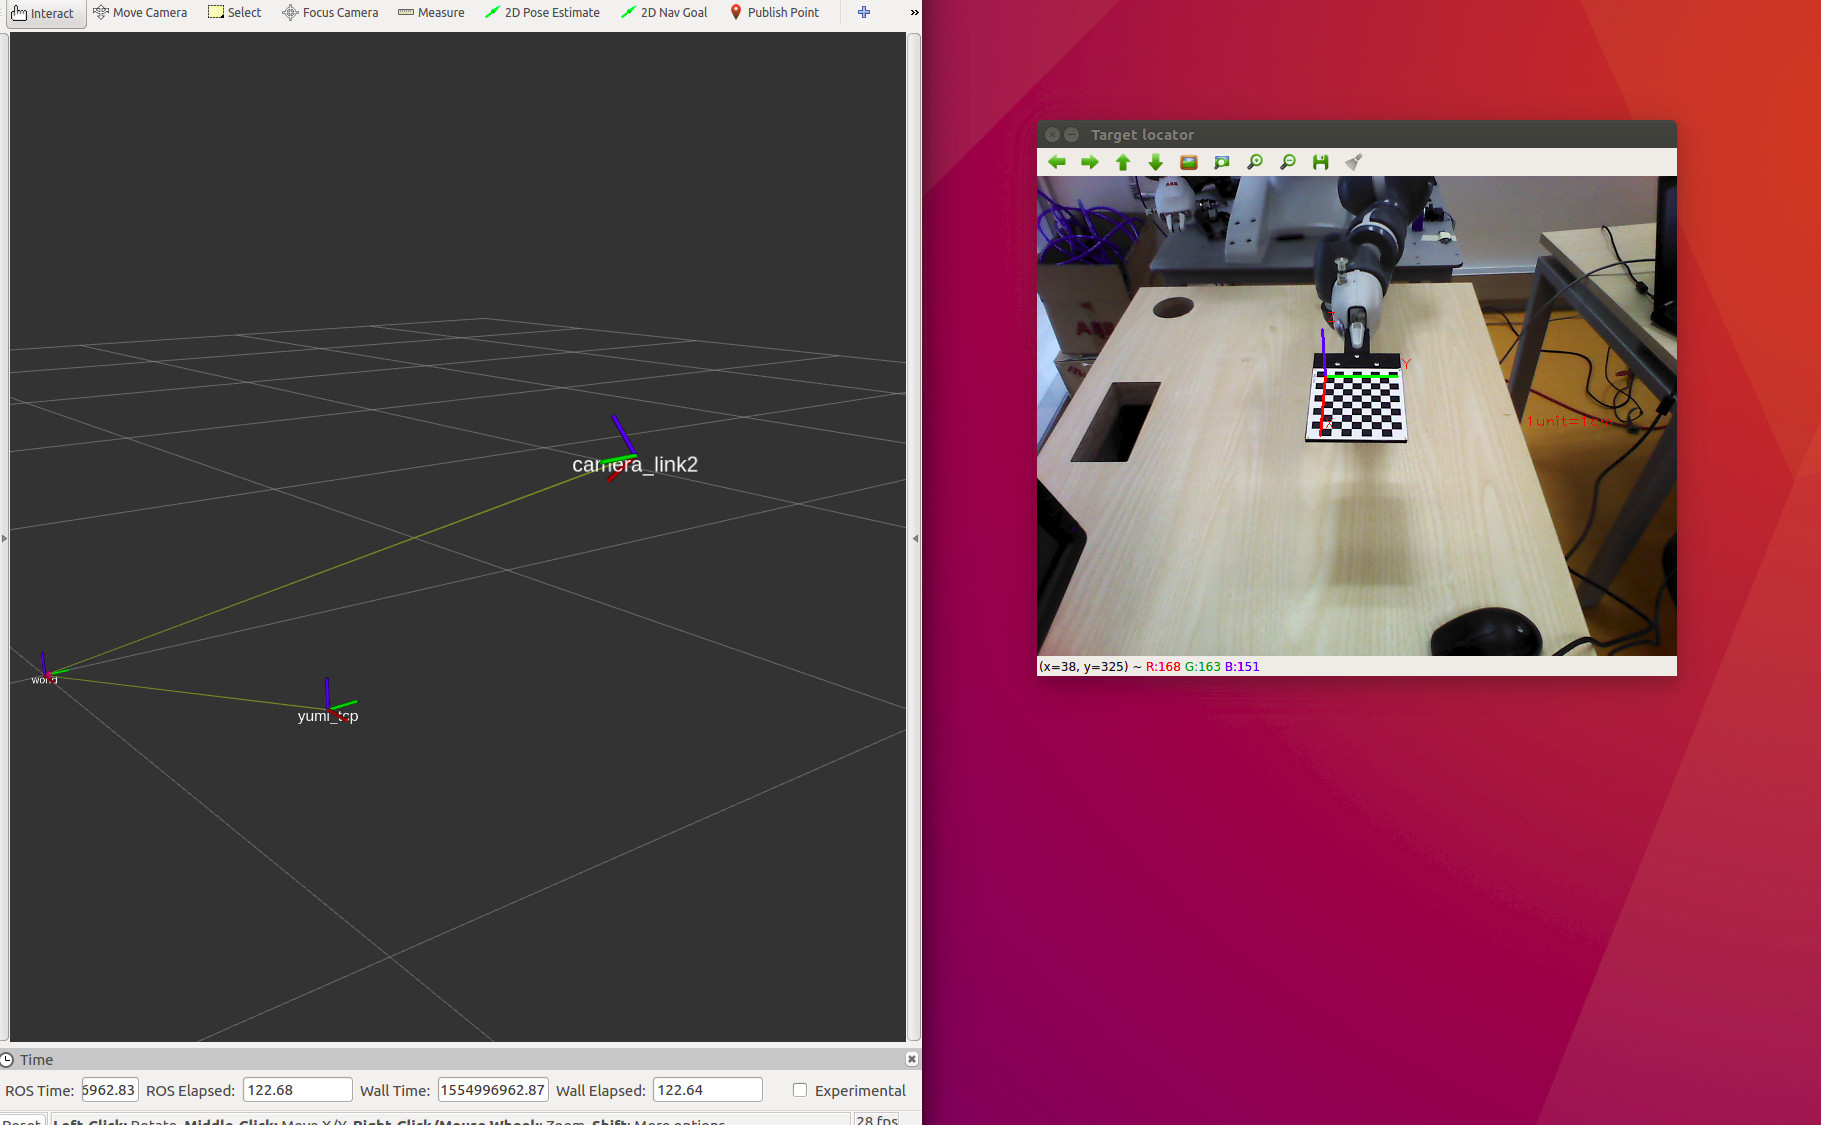
\includegraphics[clip,width=0.6\columnwidth]{images/ext2.jpg}
}
\end{center}
\caption{Setup for the Validation Test with a Constant Orientation}
\label{setupext}
\end{figure}



%%%%%%%%%
\begin{figure}[htp]
\begin{center}
{
  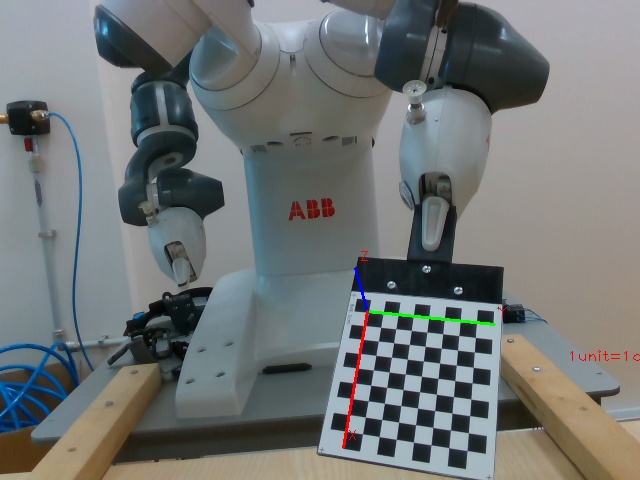
\includegraphics[clip,width=0.6\columnwidth]{images/ext3.jpg}
}
\end{center}
\caption{Setup for the Validation Test with Tilting Motion}
\label{setupext}
\end{figure}
